\begin{figure}[htbp]
\begin{center}
  \rotatebox{90}{%
    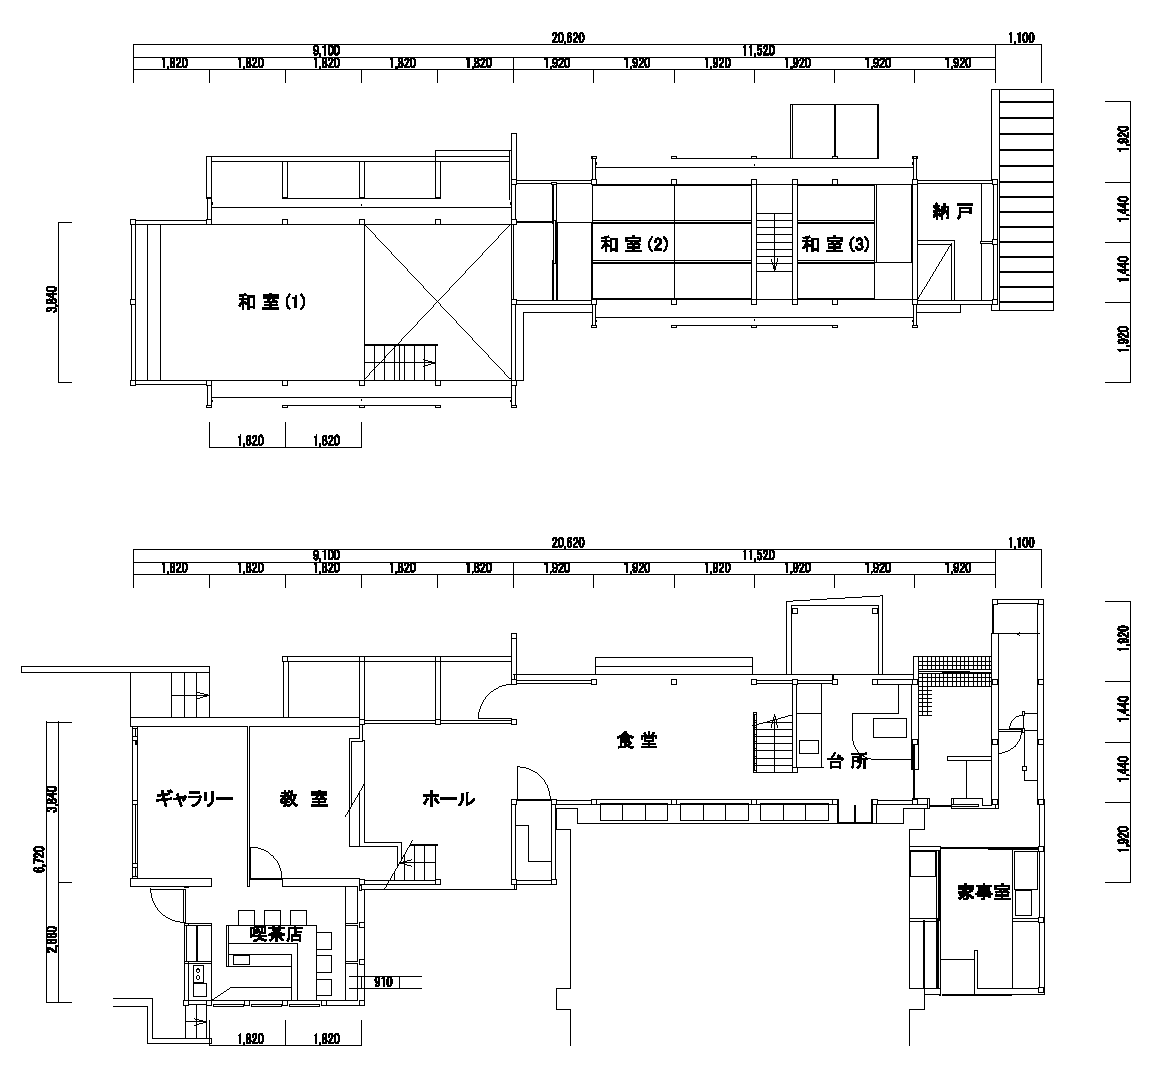
\includegraphics[height=\textwidth]{%
      Bido/1997-1998-15houses/EPS/misawa-y.eps}}
  \caption{$B?aED(BMI$BE!(B}
  \label{fig:Suita-Misawa}
\end{center}
\end{figure}

\begin{figure}[htbp]
\begin{center}
  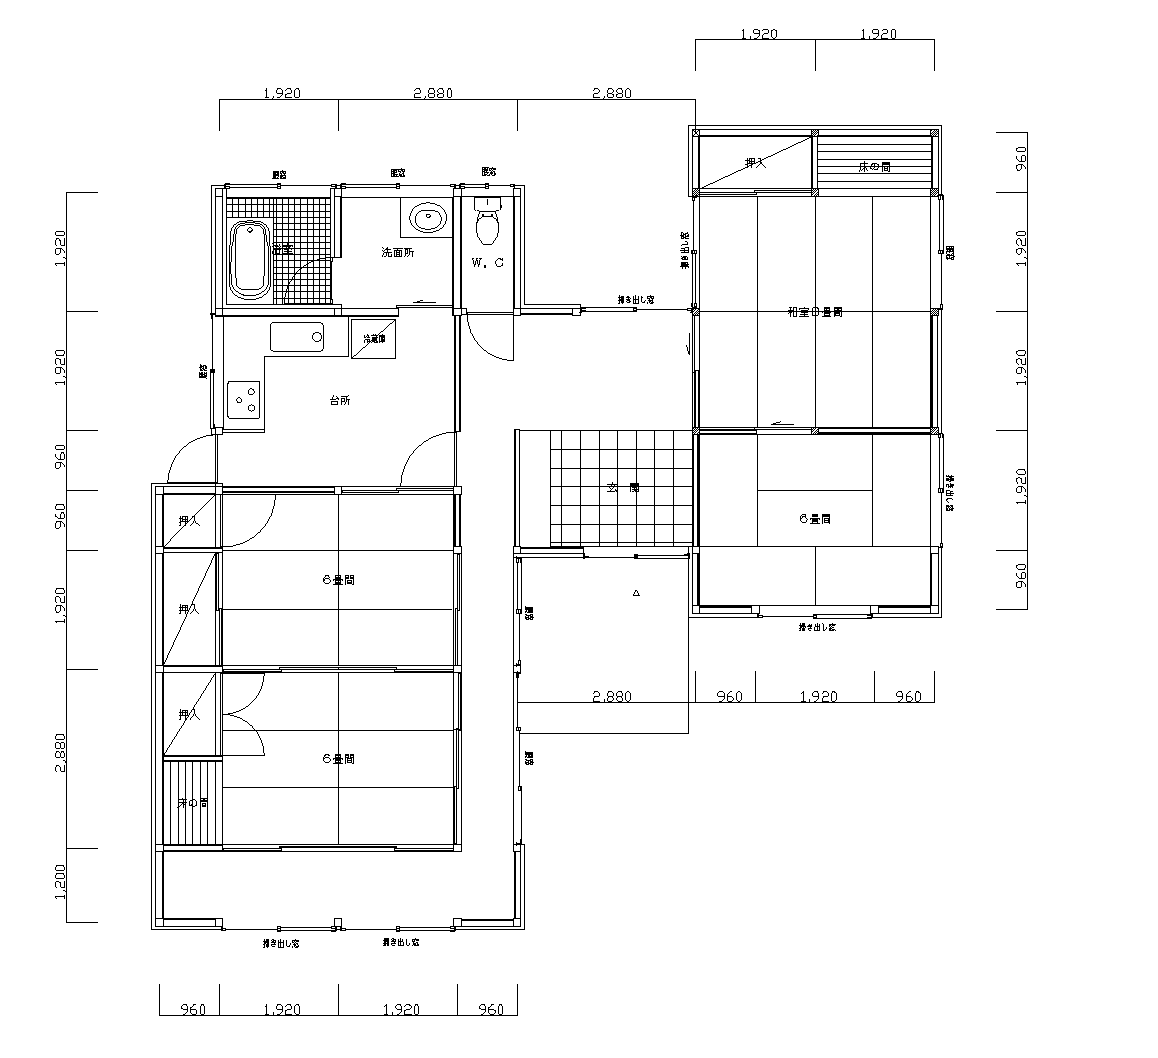
\includegraphics[width=.9\textwidth]{%
    Bido/1997-1998-15houses/EPS/ootsuka.eps}
  \caption{$B?aED(BO$BE!(B}
  \label{fig:Suita-Otsuka}
\end{center}
\end{figure}

\begin{figure}[htbp]
\begin{center}
  \rotatebox{90}{%
  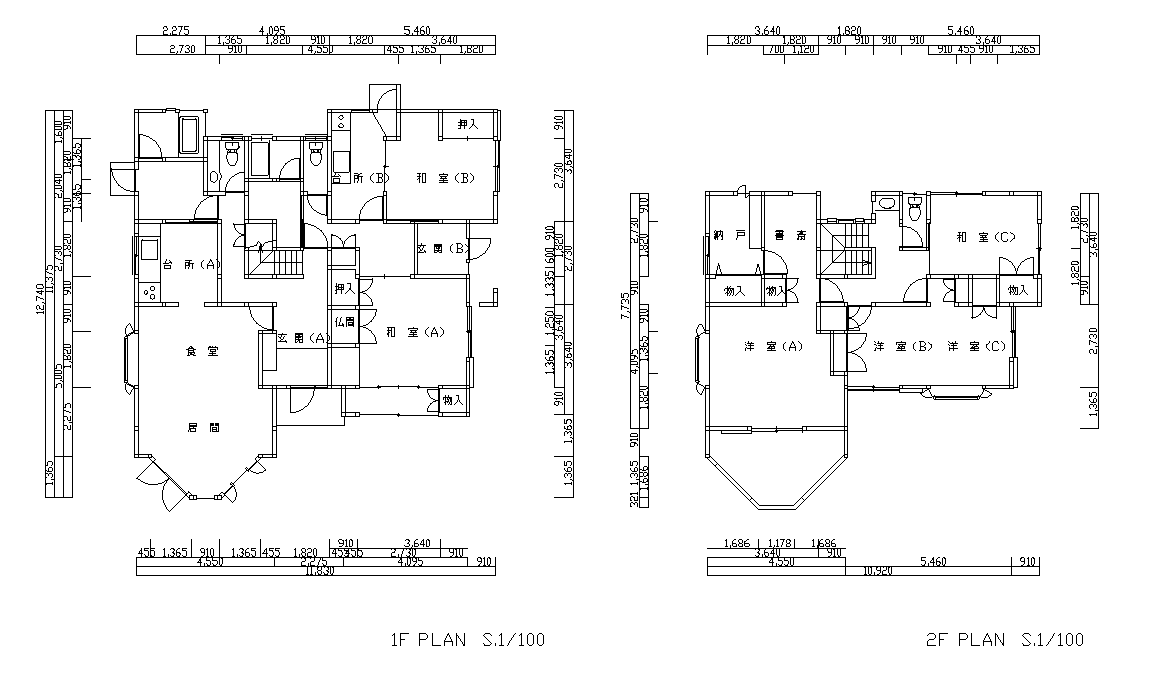
\includegraphics[width=.9\textheight]{%
    Bido/1997-1998-15houses/EPS/shimazaki.eps}}
  \caption{$B?aED(BSI$BE!(B}
  \label{fig:Suita-Shimazaki}
\end{center}
\end{figure}

\begin{figure}[htbp]
\begin{center}
  \rotatebox{90}{%
  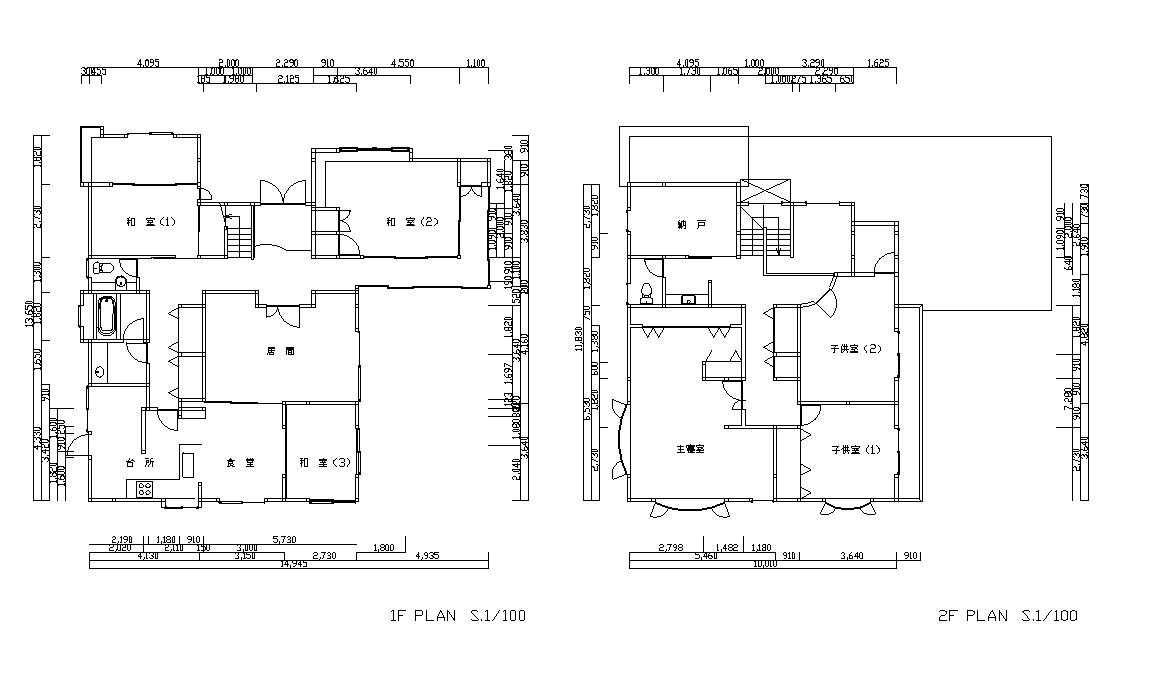
\includegraphics[width=.9\textheight]{%
    Bido/1997-1998-15houses/EPS/kinoshita.eps}}
  \caption{$B?aED(BKI$BE!(B}
  \label{fig:Suita-Kinoshita}
\end{center}
\end{figure}

\begin{figure}[htbp]
\begin{center}
  \rotatebox{90}{%
  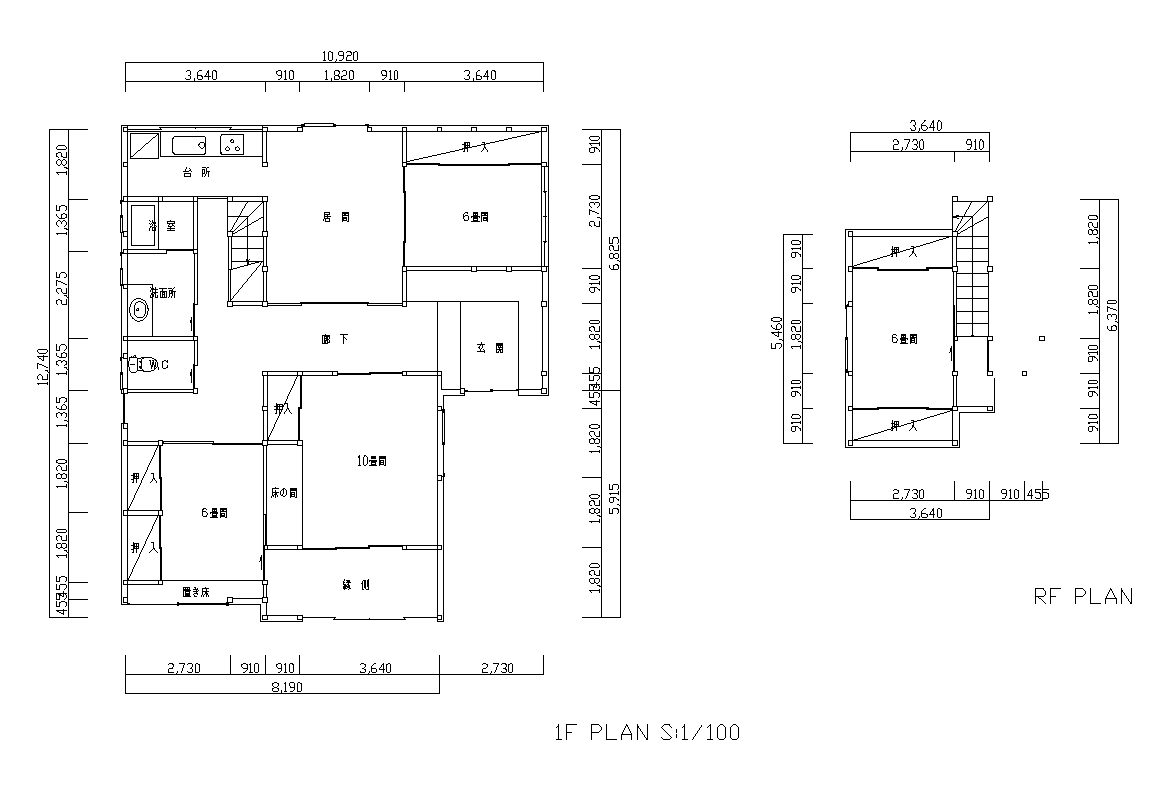
\includegraphics[width=.95\textheight]{%
    Bido/1997-1998-15houses/EPS/yamamoto.eps}}
  \caption{$BKgJ}(BYA$BE!(B}
  \label{fig:Hirakata-Yamamoto}
\end{center}
\end{figure}

\begin{figure}[htbp]
\begin{center}
  \rotatebox{90}{%
  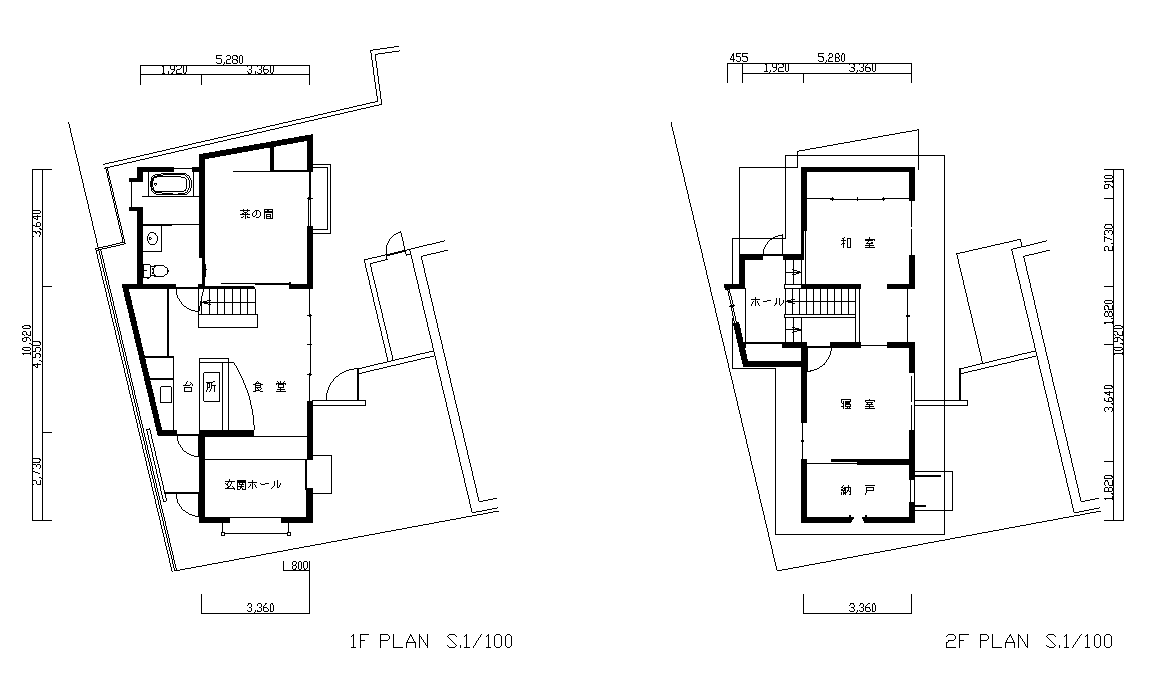
\includegraphics[width=.95\textheight]{%
    Bido/1997-1998-15houses/EPS/misawa-k.eps}}
  \caption{$B:eFn(BMI$BE!(B}
  \label{fig:Hannan-Misawa}
\end{center}
\end{figure}

\begin{figure}[htbp]
\begin{center}
  \rotatebox{90}{%
  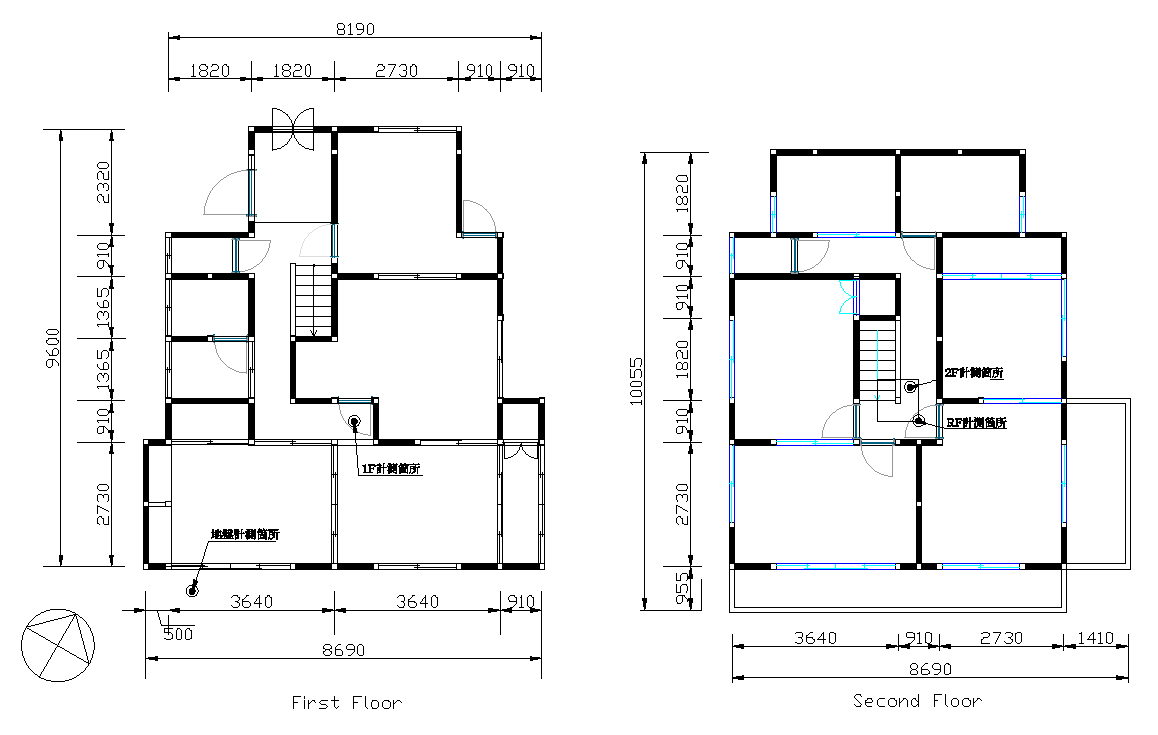
\includegraphics[width=.95\textheight]{%
    Bido/1997-1998-15houses/EPS/SUMIKURA.eps}}
  \caption{$B:eFn(BKA$BE!(B}
  \label{fig:Hannan-Kobata}
\end{center}
\end{figure}

\begin{figure}[htbp]
\begin{center}
  \rotatebox{90}{%
  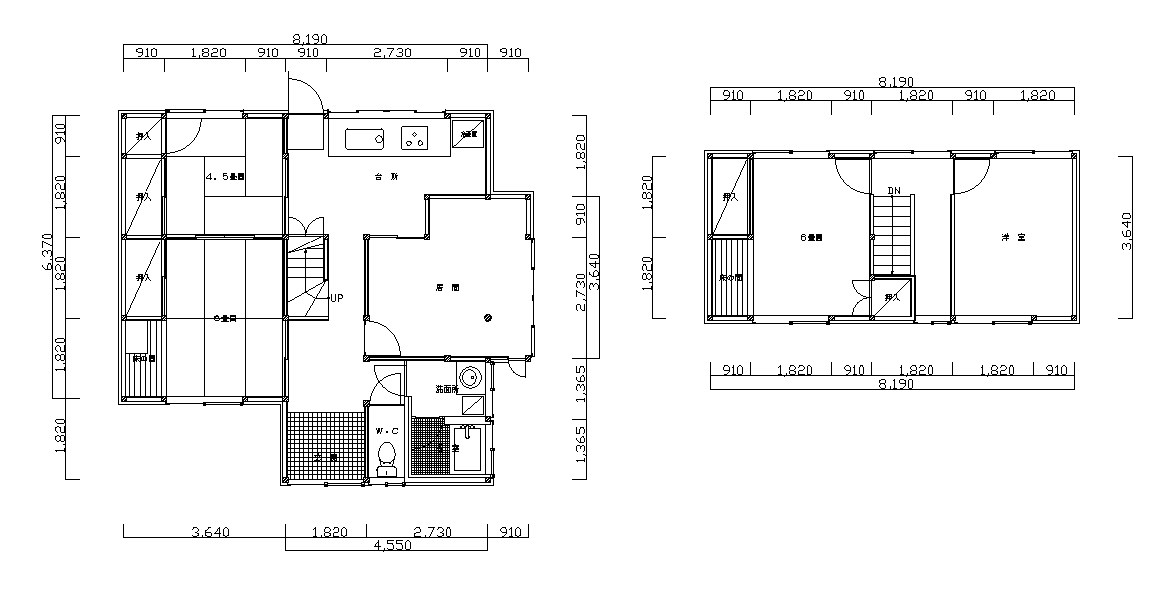
\includegraphics[width=.95\textheight]{%
    Bido/1997-1998-15houses/EPS/kodai.eps}}
  \caption{$B:eFn(BKO$BE!(B}
  \label{fig:Hannan-Kodai}
\end{center}
\end{figure}

\begin{figure}[htbp]
\begin{center}
  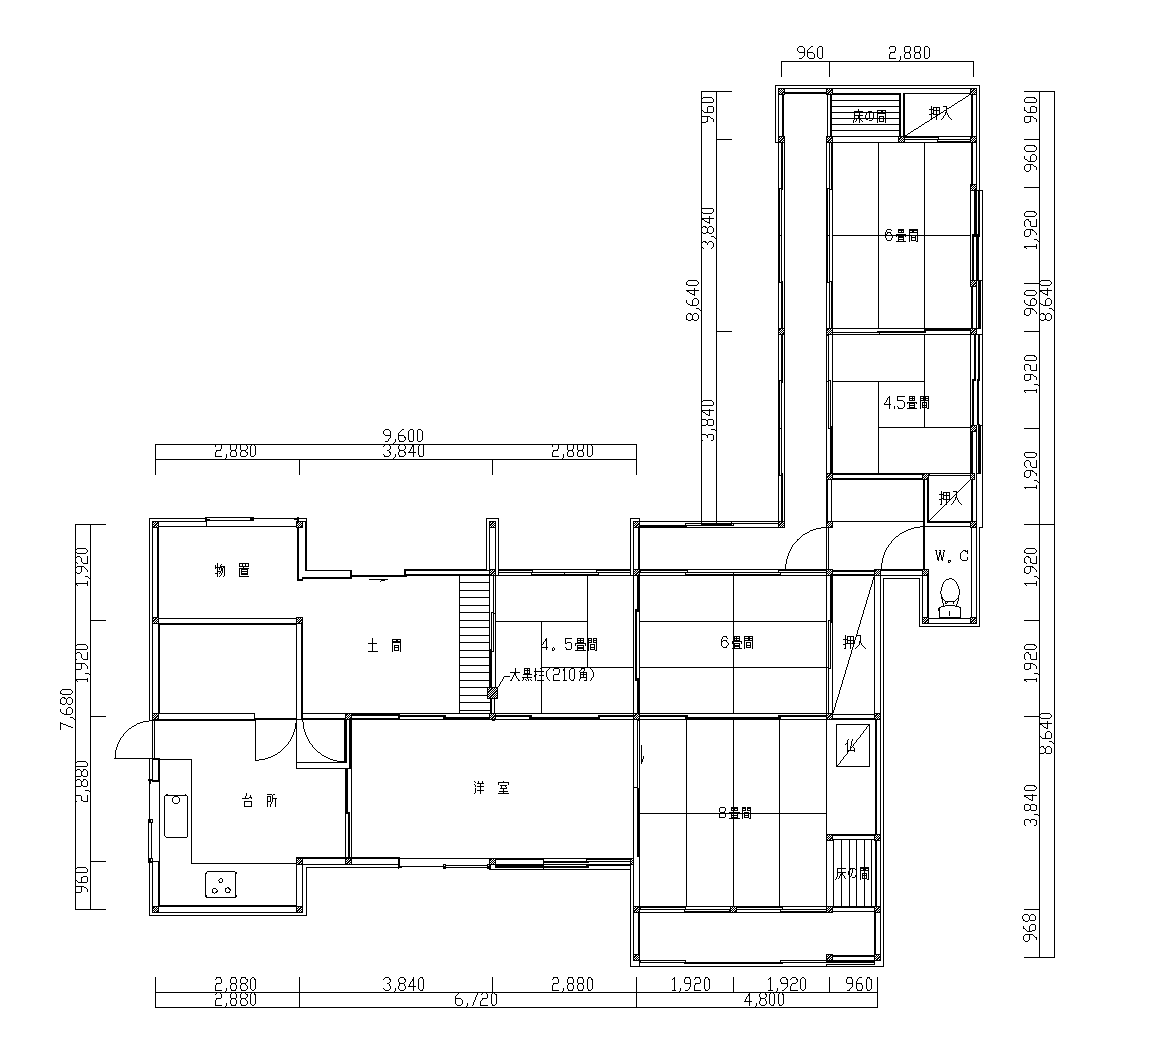
\includegraphics[width=\textwidth]{%
    Bido/1997-1998-15houses/EPS/arichi.eps}
  \caption{$B@tFn(BAR$BE!(B}
  \label{fig:Sennan-Arichi}
\end{center}
\end{figure}

\begin{figure}[htbp]
\begin{center}
  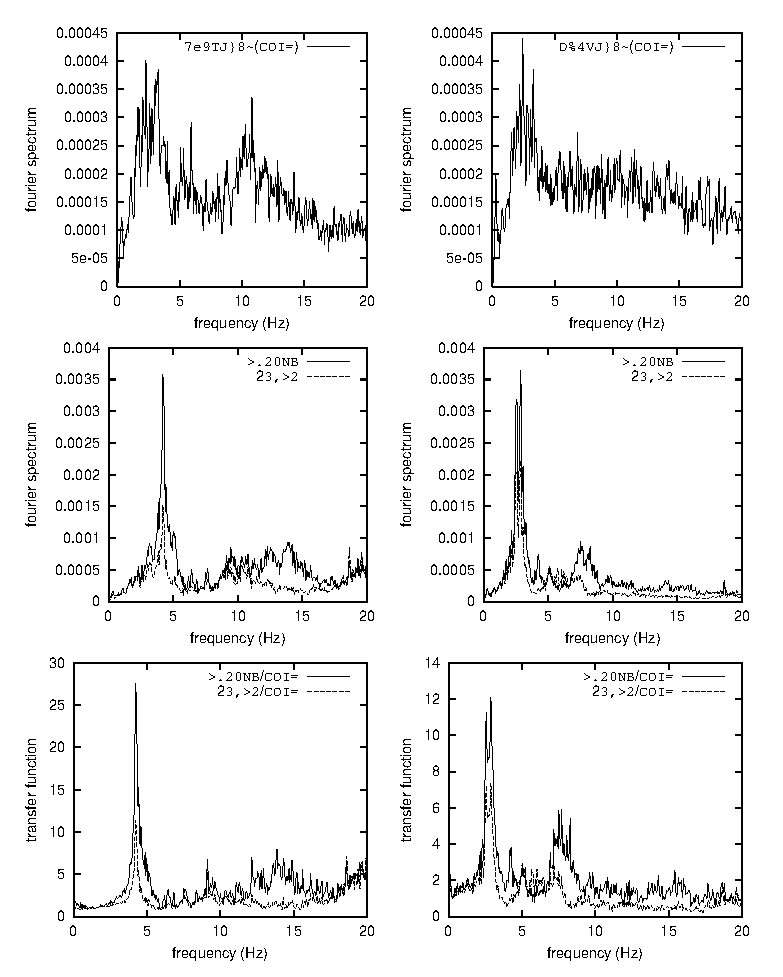
\includegraphics[width=\textwidth]{%
    Bido/1997-1998-15houses/EPS/Suzuki.eps}
  \caption{$BBg:e(BSU$BE!(B}
  \label{fig:Osaka-Suzuki}
\end{center}
\end{figure}

\begin{figure}[htbp]
\begin{center}
  \rotatebox{90}{%
  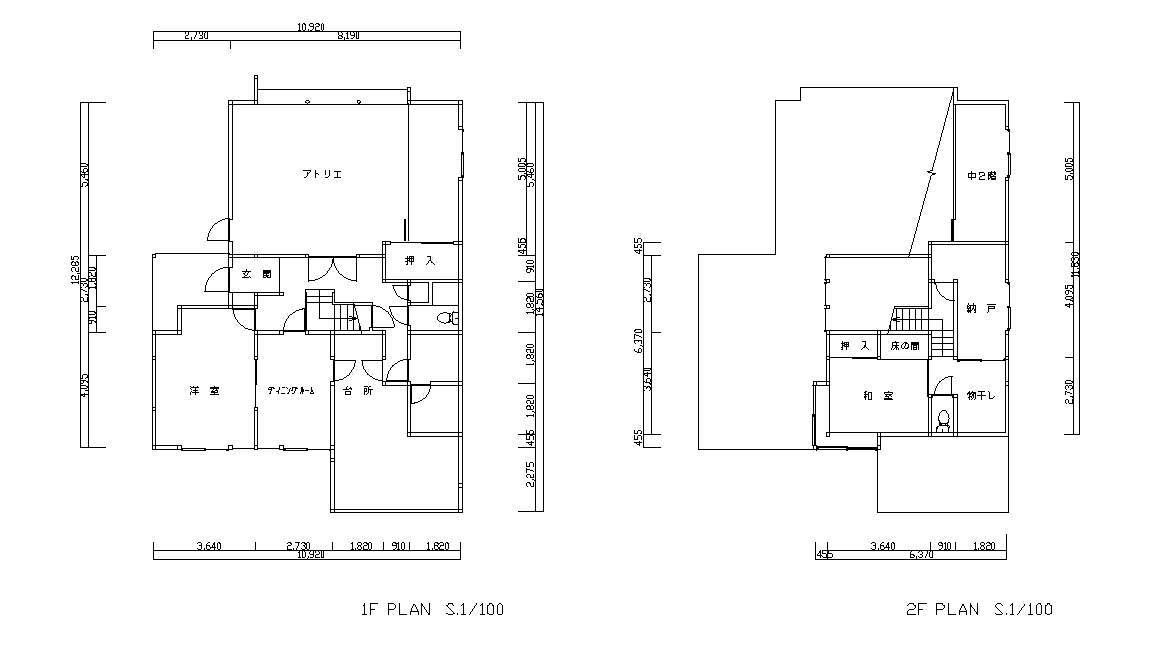
\includegraphics[width=.95\textheight]{%
    Bido/1997-1998-15houses/EPS/aoto.eps}}
  \caption{$BBg:e(BAO$BE!(B}
  \label{fig:Osaka-Aoto}
\end{center}
\end{figure}

\begin{figure}[htbp]
\begin{center}
  \rotatebox{90}{%
  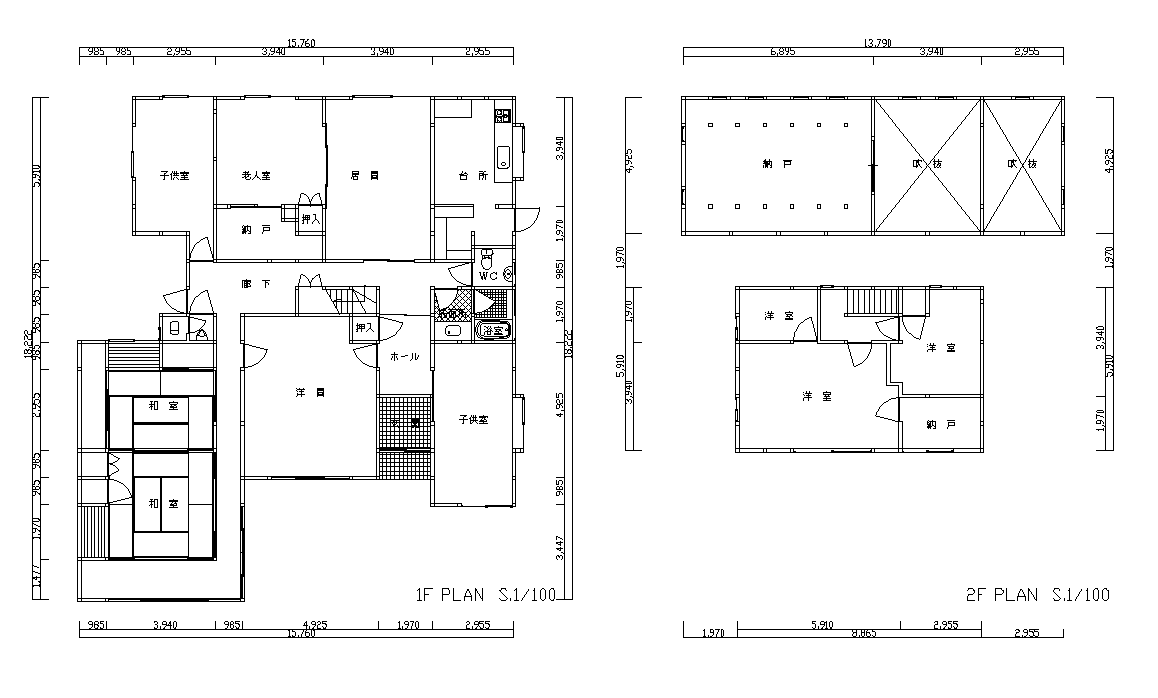
\includegraphics[width=.95\textheight]{%
    Bido/1997-1998-15houses/EPS/yasufuku.eps}}
  \caption{$B?@8M(BYA$BE!(B}
  \label{fig:Kobe-Yasufuku}
\end{center}
\end{figure}

\begin{figure}[htbp]
\begin{center}
  \rotatebox{90}{%
  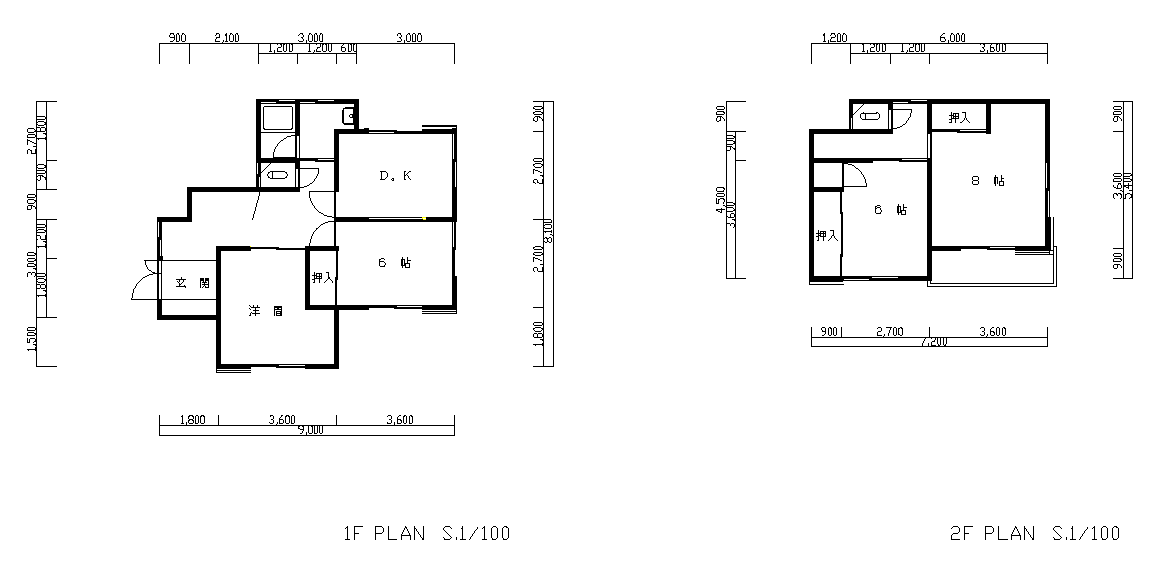
\includegraphics[width=.95\textheight]{%
    Bido/1997-1998-15houses/EPS/shirai.eps}}
  \caption{$B?@8M(BSI$BE!(B}
  \label{fig:Kobe-Shirai}
\end{center}
\end{figure}

\begin{figure}[htbp]
\begin{center}
  \rotatebox{90}{%
  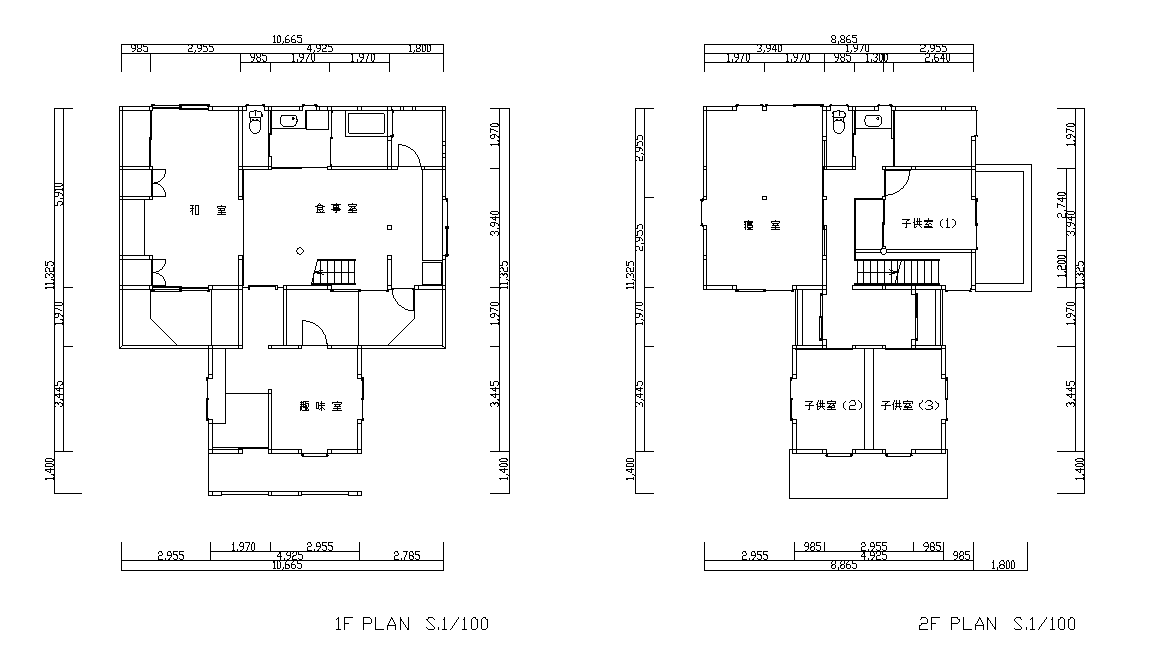
\includegraphics[width=.95\textheight]{%
    Bido/1997-1998-15houses/EPS/kobata.eps}}
  \caption{$B?@8M(BMO$BE!(B}
  \label{fig:Kobe-Mo}
\end{center}
\end{figure}

\newpage{}

\begin{figure}[htbp]
\begin{center}
  \rotatebox{90}{%
  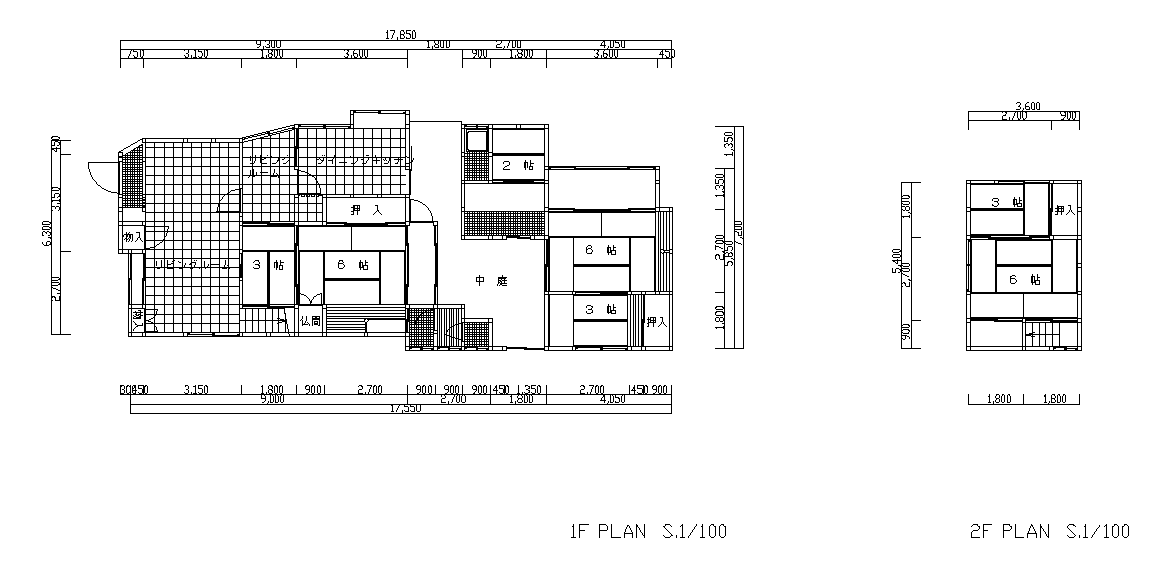
\includegraphics[width=.95\textheight]{%
    Bido/1997-1998-15houses/EPS/nagata.eps}}
  \caption{$BLg??(BNA$BE!(B}
  \label{fig:Kadoma-Na}
\end{center}
\end{figure}

%%% Local Variables: 
%%% mode: latex
%%% TeX-master: "/home/nakaji/paper/phD/paper"
%%% End: 
